% !TeX program = pdflatex
\documentclass[russian,utf8,simple]{eskdtext}

% packages
%
% Тестовое наполнение текстом
% При написании работы - удалить пакет и комманды \lipsum
\usepackage{lipsum}
%
\usepackage{graphicx}
\usepackage{datetime}
\usepackage{enumitem} % for lists
\usepackage{ulem} % for underlining
\usepackage{lastpage} % Number of pages
\usepackage{hyperref} % Links in pdf

% setup
\newcommand{\FrontPageDepartment}{ИТ} %Факультет
\newcommand{\FrontPageSubdepartment}{САПР} %Кафедра
\newcommand{\WorkType}{Лабораторная работа №4} %Тип работы (заголовок)
\newcommand{\Subject}{Инструментальные средства разработки программного обеспечения} %по ... родительный падеж
\newcommand{\Topic}{Разработка приложения на языке Python с использованием QtQML} %Тема
\newcommand{\Professor}{Пугин~Е.~В.} %Руководитель
\newcommand{\Student}{Балашова~О.~В.} %Студент
\newcommand{\Group}{ПКС-115} %Группа
\newcommand{\FrontPageDate}{\ddmmyyyydate\today} %Дата

\ESKDsignature{МИВУ 09.02.03} % Код специальности и тип работы

% eskdx setup
\ESKDletter{}{У}{}
\ESKDtitle{\WorkType

\Topic}
\ESKDchecker{\Professor}
\ESKDauthor{\Student}
\ESKDcolumnIX{МИ ВлГУ\\ \Group}

\addto\captionsrussian{\def\refname{Список использованных источников}}
\sloppy % split long lines

% graphics path
\graphicspath{{src/img/}}


% verbatim setup
\newcommand{\verbatimFont}{
\fontsize{10pt}{12pt}\selectfont
\baselineskip=1em
}


% workaround for regression in babel package on linux
\providecommand{\No}{\textnumero}


% remove vertical space from lists
%\renewcommand{\alph}[1]{\asbuk{#1}} % костыль для кирилической нумерации вместо латинской
\setlist{nolistsep} % убираем дополнительные вертикальные отступы вокруг списков
\setenumerate[1]{label=\arabic*), fullwidth, itemindent=\parindent,  listparindent=\parindent}
\setenumerate[2]{label=\arabic*), fullwidth, itemindent=\parindent, listparindent=\parindent, leftmargin=\parindent}
\setitemize{fullwidth, itemindent=\parindent, listparindent=\parindent}

% main document
\begin{document}
% Титул
\ESKDthisStyle{title}
\newlength{\frontpagefk} % Ширина поля Факультет/Кафедра
\setlength{\frontpagefk}{6cm}
\newlength{\frontpagerb} % Ширина надписей Руководитель/Студент и пр. под темой
\setlength{\frontpagerb}{6cm}
\newlength{\frontpagerbspace} % ??? (do not remove)
\setlength{\frontpagerbspace}{1cm}
\newlength{\FrontPageSubjSpace} % Ширина пробела до и после названия предмета
\setlength{\FrontPageSubjSpace}{1cm}
\newlength{\FrontPageTopicSpace} % Ширина пробела до и после темы
\setlength{\FrontPageTopicSpace}{0.5cm}

\thispagestyle{empty}
\begin{center}
{
\vspace*{-1.5cm}
\baselineskip=1.3em
{\small Министерство образования и науки Российской Федерации}\\
\textbf{Муромский институт (филиал)}\\
{\footnotesize федерального государственного бюджетного образовательного учреждения\\
высшего профессионального образования}\\
\textbf{<<Владимирский государственный университет\\
имени Александра Григорьевича и Николая Григорьевича\\
Столетовых>>\\
(МИВлГУ)\\}
}

\bigskip
\begin{tabular}{l c}
\textbf{Факультет}&\underline{\makebox[\frontpagefk]{\FrontPageDepartment}}\\
\textbf{Кафедра}&\underline{\makebox[\frontpagefk]{\FrontPageSubdepartment}}\\
\end{tabular}

\vspace{\fill}
\begin{Huge}
\textbf{\textsl{\WorkType}}
\end{Huge}

\vspace{\fill}
по \underline{\makebox[\FrontPageSubjSpace]{}\Subject\makebox[\FrontPageSubjSpace]{}}

\smallskip
\parbox{15cm}{\centering{Тема: \uline{\makebox[\FrontPageTopicSpace]{}\Topic\makebox[\FrontPageTopicSpace]{}}}}

\vspace{\fill}

\begin{flushright}
\makebox[\frontpagerb][c]{
\makebox[\frontpagerb][l]{Руководитель}\hspace{\frontpagerbspace}}

\smallskip
\makebox[\frontpagerb][c]{
\raisebox{-\baselineskip}{\shortstack{\underline{\makebox[\frontpagerb][l]{\Professor}}\\
\begin{footnotesize}
(фамилия, инициалы)
\end{footnotesize}}}\hspace{\frontpagerbspace}}

\bigskip
\makebox[\frontpagerb][c]{
\raisebox{-\baselineskip}{\shortstack{\underline{\makebox[\frontpagerb][l]{}}\\
\begin{footnotesize}
(подпись)\hfill(дата)
\end{footnotesize}}}\hspace{\frontpagerbspace}}

\newcommand{\frontpagerbstudent}[2]{ %
\makebox[\frontpagerb]{ %
\raisebox{-\baselineskip}{\shortstack{#1\ \underline{\makebox[\frontpagerb-\widthof{#1\ }][c]{#2}}\\
\begin{footnotesize}
\makebox[\widthof{#1\ }][c]{}\makebox[\frontpagerb-\widthof{#1\ }][c]{(группа)}
\end{footnotesize}}}\hspace{\frontpagerbspace}}
}

\bigskip
\makebox[\frontpagerb][c]{\frontpagerbstudent{Студент}{\Group}}

\smallskip
\makebox[\frontpagerb][c]{
\raisebox{-\baselineskip}{\shortstack{\underline{\makebox[\frontpagerb][l]{\Student}}\\
\begin{footnotesize}
(фамилия, инициалы)
\end{footnotesize}}}\hspace{\frontpagerbspace}}

\renewcommand{\dateseparator}{.}

\bigskip
\makebox[\frontpagerb][c]{
\raisebox{-\baselineskip}{\shortstack{\underline{\makebox[\frontpagerb][r]{\FrontPageDate}}\\
\begin{footnotesize}
(подпись)\hfill(дата)
\end{footnotesize}}}\hspace{\frontpagerbspace}}

\end{flushright}

\vspace{\fill}
Муром \the\year
\vspace*{-1cm}
\end{center}
\newpage



% Основной текст
\ESKDthisStyle{formII}
\begin{center}
{\WorkType}
\\
Тема: {\Topic}
\\
Цель: Создание простейшей программы на языке C\# с использованием WPF. 
\end{center}
Задание:
Создание калькулятора.

Ход выполнения:
\begin{center}
Программа:
\end{center}
\begin{verbatim}
namespace WpfApp1
{
/// <summary>
/// Логика взаимодействия для MainWindow.xaml
/// </summary>
public partial class MainWindow : Window
{
public MainWindow()
{
InitializeComponent();
}

public double c = 0;
bool bplus = false, bminus = false, bumnoj = false, bdelen = false, bpoint = false;

private void Button_Click(object sender, RoutedEventArgs e)
{
texb.Text += 0;
}

private void one_Click(object sender, RoutedEventArgs e)
{
texb.Text += 1;
}

private void two_Click(object sender, RoutedEventArgs e)
{
texb.Text += 2;
}

private void three_Click(object sender, RoutedEventArgs e)
{
texb.Text += 3;
}

private void four_Click(object sender, RoutedEventArgs e)
{
texb.Text += 4;
}

private void five_Click(object sender, RoutedEventArgs e)
{
texb.Text += 5;
}

private void six_Click(object sender, RoutedEventArgs e)
{
texb.Text += 6;
}

private void seven_Click(object sender, RoutedEventArgs e)
{
texb.Text += 7;
}

private void eight_Click(object sender, RoutedEventArgs e)
{
texb.Text += 8;
}

private void nine_Click(object sender, RoutedEventArgs e)
{
texb.Text += 9;
}

private void point_Click(object sender, RoutedEventArgs e)
{
texb.Text += ',';
point.IsEnabled = false;
}

private void C_Click(object sender, RoutedEventArgs e)
{
if (texb.Text.Length != 0) 
texb.Text = texb.Text.Substring(0, texb.Text.Length - 1);
for (int i = 0; i < texb.Text.Length; i++)
if (texb.Text[i] == ',')
{
bpoint = true;
break;
}
if (bpoint == true)
point.IsEnabled = false;

else
point.IsEnabled = true;


}

private void CE_Click(object sender, RoutedEventArgs e)
{
texb.Text = "";
}

private void delenie_Click(object sender, RoutedEventArgs e)
{
bdelen = true;
c = Convert.ToDouble(texb.Text);
texb.Text = "";
}

private void umnojenie_Click(object sender, RoutedEventArgs e)
{
bumnoj = true;
c = Convert.ToDouble(texb.Text);
texb.Text = "";
}

private void minus_Click(object sender, RoutedEventArgs e)
{
bminus = true;
c = Convert.ToDouble(texb.Text);
texb.Text = "";
}

private void ravno_Click(object sender, RoutedEventArgs e)
{
if (bplus == true)
{
c += Convert.ToDouble(texb.Text);
bplus = false;
}

else
if (bminus == true)
{
c -= Convert.ToDouble(texb.Text);
bminus = false;
}

else
if (bumnoj == true)
{
c *= Convert.ToDouble(texb.Text);
bumnoj = false;
}

else
if (bdelen == true)
{
c /= Convert.ToDouble(texb.Text);
bdelen = false;
}

else
c = Convert.ToDouble(texb.Text);

texb.Text = Convert.ToString(c);              
}

private void plus_Click(object sender, RoutedEventArgs e)
{
bplus = true;
c = Convert.ToDouble(texb.Text);
texb.Text = "";

}
}
}
\end{verbatim}
Изображен код программы калькулятор.
\begin{center}
Результат работы программы:
\end{center}

\begin{figure}[h]
	\centering
	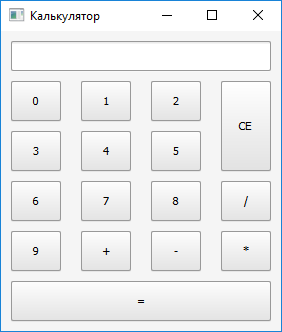
\includegraphics[scale=1]{s1}

	\label{fig:s1}
\end{figure}
Изображен результат работы программы.

Вывод: Создала простейшию программу на языке C\# с использованием WPF. 




\newpage
\end{document}